%% LyX 2.2.3 created this file.  For more info, see http://www.lyx.org/.
%% Do not edit unless you really know what you are doing.
\documentclass[english]{article}
\usepackage[T1]{fontenc}
\usepackage[latin9]{luainputenc}
\usepackage{graphicx}
\usepackage{babel}
\begin{document}

\section{Circuito no inversor}

\begin{figure}
\begin{centering}
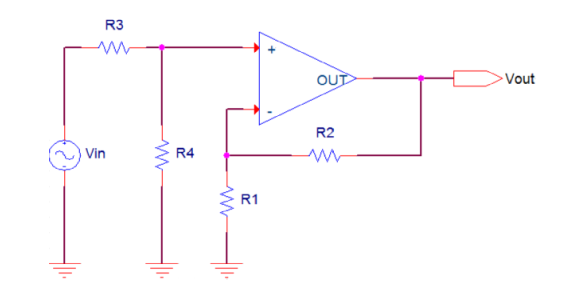
\includegraphics[scale=0.5]{Resources1b/circuit}
\par\end{centering}
\caption{Circuito B}

\end{figure}

\[
H(s)=\frac{R_{4}\omega_{p}a_{0}\left(R_{1}+R_{2}\right)}{\left(R_{3}-R_{4}\right)\left(R_{1}\omega_{p}a_{0}+\left(R_{1}+R_{2}\right)\left(\omega_{p}+s\right)\right)}
\]

\[
H(s)=\frac{414\,10^{9}}{110\,10^{3}s+47\,10^{9}}\,\,\,Caso\,1
\]

\[
H(s)=\frac{75\,10^{9}}{20\,10^{3}s+47\,10^{9}}\,\,\,Caso\,2
\]

\[
H(s)=\frac{414\,10^{9}}{110\,10^{3}s+471\,10^{9}}\,\,\,Caso\,3
\]

\end{document}
